\chapter{Architetture di Base}

Quando si parla di Deep Learning, si usano spesso delle strutture grafiche, aggiungendo dei livelli di astrazione, per poter semplificare la comprensione delle architetture complesse, queste strutture prendono il nome di \textbf{Grafi Computazionali}. La rappresentazione grafica di alcuni dei modelli più complessi, permette di comprendere al meglio come vengono implementate alcune nuove tecniche. Adesso vedremo, semplici implementazioni, per dare un'idea di utilizzo, e lasciare a chi legge, la possibilità di adottarle nei propri progetti.

\section{Moduli moltiplicativi}
Iniziamo da delle architetture semplici: i moduli moltiplicativi. Creiamo immediatamente un collegamento con questi moduli, sfruttando un esempio pratico. Nel processo di backpropagation essi vengono utilizzati, poiché si può effettuare tale processo, rispetto agli input, o rispetto ai pesi. La differenza fra operare rispetto agli uno o gli altri si trova nell'impossibilità di imparare direttamente i pesi, come avviene per gli input. In molti hanno pensato cosa succederebbe nel caso in cui i pesi fossero gli output di un'altra Rete Neurale, questa possibilità viene sfruttata tramite i moduli moltiplicativi.

\begin{equation}
    s_i = \sum_{j}w_{ij}x_{j}\,:\, w_{ij}=\sum_ku_{ijk}z_k \Rightarrow s_i=\sum_{jk}u_{ijk}z_kx_j
    \label{eq:weightAsInput}
\end{equation}

Come vediamo nella formula di cui sopra, possiamo notare come, essa sia una sostituzione semplice, ottenendo comunque un risultato desiderato, senza modificare il senso dell'operazione. Questa semplice sostituzione, è stata adottata in molti contesti di Deep Learning.
\begin{figure}[htbp]
    \centering
    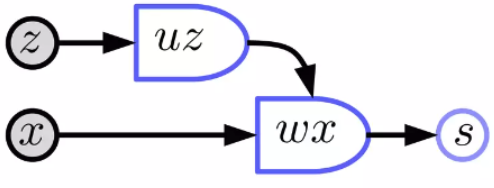
\includegraphics[width=0.4\linewidth]{figure/WeightAsInput.png}
    \caption{Grafo computazionale corrispettivo all'equazione~\ref{eq:weightAsInput}}
    \label{fig:wai}
\end{figure}

Se avessimo una Rete Neurale che si occupa del controllo dei pesi, saremmo in grado di crearne una nuova con una semplice variazione di essi, potendo persino ampliarne la portata riuscendo a controllarne molte reti con una a supervisionare. Questo non è un lavoro semplice, dovremmo effettuare delle limitazioni per non incorrere in problematiche di esplosione della rete stessa. Dunque la rete neurale al di sopra delle altre, funziona come un "controllore", pesando di più una sottorete piuttosto che un'altra (Figura~\ref{eq:attentionMod}). Questo meccanismo si implementa adoperando la funzione \textbf{SoftMax}, che tratteremo più avanti, essa ci permette di calcolare nuovi pesi ed effettuare un'attivazione. Questa architettura prende il nome di \textbf{Modulo dell'attenzione}, dando più o meno importanza in base all'input ricevuto alle singole reti neurali.

\begin{equation}
    s_i = \sum_jw_jx_{ij} \,:\,w_j=\frac{e^{z_{j}}}{\sum_ke^{z_k}}
    \label{eq:attentionMod}
\end{equation}

\begin{figure}[htbp]
    \centering
    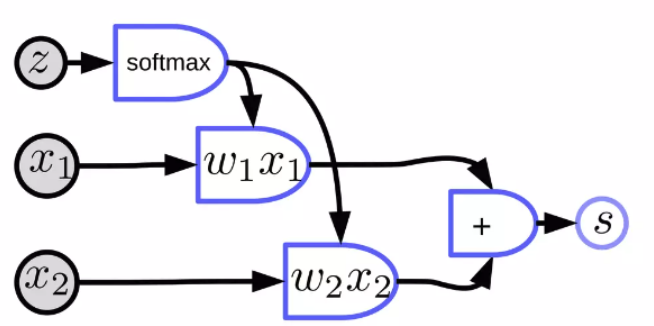
\includegraphics[width=0.4\linewidth]{figure/AttentionModule.png}
    \caption{Grafo computazionale rappresentante il Modulo dell'attenzione, in cui ci sono più reti, controllate da una singola, la quale da più o meno importanza alle sottoreti in base all'input ricevuto.}
    \label{fig:AttentionMod}
\end{figure}

\subsubsection{Mixture of Experts}
L'idea che stiamo analizzando, inserendo più reti neurali in un'unica architettura, prende il nome di \textbf{Mixture of Experts}, partendo da una semplice rete neurale con $x_1$ e $x_2$ come ingressi, la estendiamo rendendola un'\textit{esperta}, creando una rete con all'interno milioni di parametri. Il modello Mixture of Experts è una rete neurale, la quale controlla diversi task, spezzati nelle singole sottoreti, selezionando su quale fare affidamento a seconda della necessità (Figura~\ref{fig:mixExp}). I modelli di linguaggio, utilizzano questa strategia, prendono in considerazione una combinazione di reti specializzate in diverse attività (es. Traduzione, riassunto, calcoli, ecc\dots). 

\begin{figure}[htbp]
    \centering
    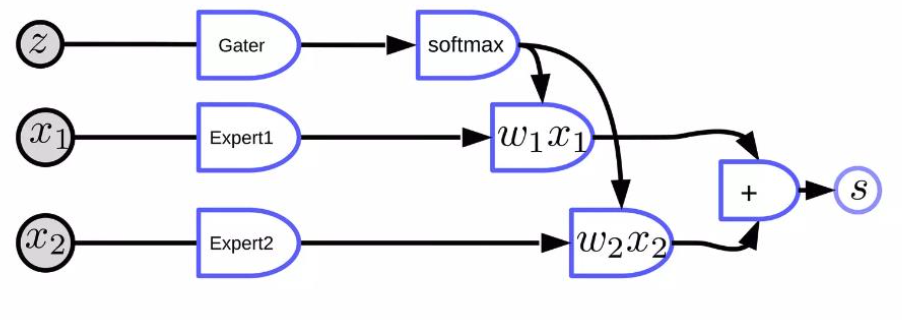
\includegraphics[width=0.5\linewidth]{figure/MixtureOfExpert.png}
    \caption{Grafo computazionale, del modello Mixture of Experts, vari modelli specializzati in compiti specifici, attivati o disattivati da un'altra rete neurale tramite l'utilizzo della funzione softmax.}
    \label{fig:mixExp}
\end{figure}

\subsubsection{Parameter Transoformation}

Un modo generale per concettualizzare architetture come la Mixture of Experts è attraverso l'idea di \textbf{Parameter Transformation}. Invece di considerare i parametri di un modello, come i pesi $W$, dei valori statici appresi una sola volta, li concepiamo come l'output dinamico di un altro modulo. In pratica, la rete impara a generare o selezionare i parametri più adatti in base al contesto fornito dall'input. L'architettura Mixture of Experts (MoE) può essere vista come un caso specifico di questo principio. In una MoE, la rete generale non crea nuovi pesi, ma seleziona quale set di parametri (quello di un "esperto") utilizzare. Differentemente la Parameter Transformation è un'operazione di selezione dinamica. Una delle applicazioni più diffuse di questo concetto è la \textit{Weight Sharing}. Questa tecnica consiste nell'utilizzare lo stesso modulo parametrico, definito da un set di pesi $w$, applicandolo ripetutamente in diverse parti di un modello o per elaborare porzioni differenti dell'input (Figura~\ref{fig:wshar}).

\begin{figure}[htbp]
    \centering
    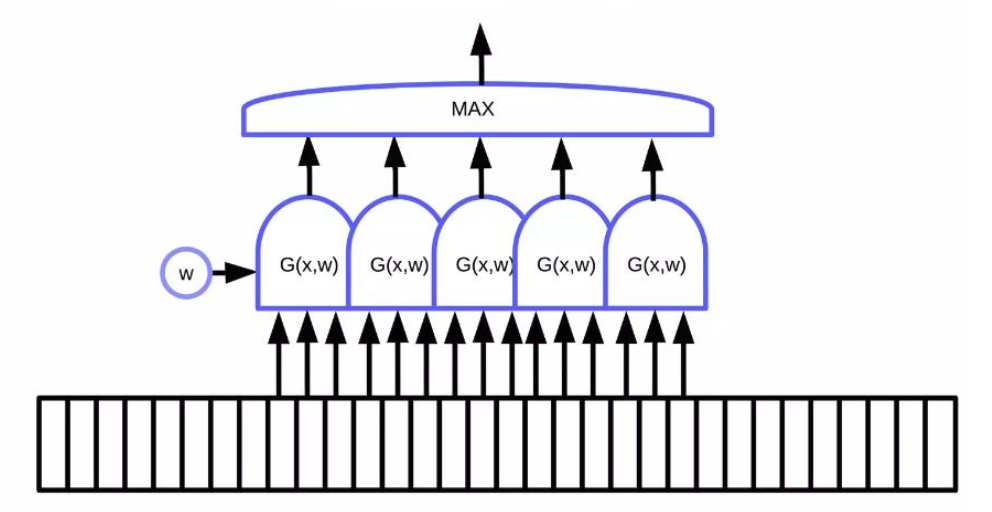
\includegraphics[width=0.65\linewidth]{figure/WeightShar.png}
    \caption{Esempio di grafo computazionale che implementa la Weight Sharing. Un unico set di parametri, il kernel $w$, riutilizzato ripetutamente dalla funzione $G$ su diverse sezioni dell'input.}
    \label{fig:wshar}
\end{figure}

Quindi si ha un modulo generatore di pesi, iniettato in diversi punti della rete principale permettendo di avere due vantaggi principali:

\begin{itemize}
    \item \textbf{Efficienza:} Invece di dover apprendere e memorizzare un set di pesi indipendente per ogni operazione, si apprende un unico e più compatto modulo che sa come generarli. Riduce drasticamente il numero totale di parametri del modello, rendendolo più leggero ed efficiente;
    \item \textbf{Generalizzazione:} Durante l'addestramento, il processo di backpropagation diventa particolarmente efficace. Se lo stesso modulo di pesi condivisi viene utilizzato in $N$ contesti diversi, esso riceverà i gradienti di errore da tutte e $N$ le funzioni di costo parziali. Questo "costringe" il modulo ad apprendere parametri che non siano specifici per un singolo compito, ma che siano abbastanza robusti da funzionare bene in tutte le situazioni. Porta a un risultato con una migliore capacità di generalizzazione.
\end{itemize}
